% SC1004 Chapter 1: Vectors & Geometry (0->100 ground-up)
\chapter{Vectors and Geometry}
\label{ch:vectors}

\begin{quote}
\emph{``A vector is not just a list of numbers --- it is an arrow that knows where to push.''} This chapter gives that arrow a home: from points on a map to $n$-dimensional space, with pictures before formulas.
\end{quote}

\noindent\fbox{\parbox{\dimexpr\linewidth-2\fboxsep-2\fboxrule}{%
\textbf{From zero: no prior linear algebra assumed.} We start with a dot on paper, then an arrow, then coordinates. Every notion --- length, angle, line, plane --- is drawn before it is defined. By the end you will do geometry with algebra.}}
\vspace{0.4em}

\section*{Learning Outcomes}
After this chapter you will be able to:
\begin{enumerate}[label=(L\arabic*)]
    \item represent vectors geometrically and algebraically in $\mathbb{R}^2$, $\mathbb{R}^3$, and $\mathbb{R}^n$;
    \item compute dot products, norms, and angles and interpret them geometrically;
    \item write parametric equations of lines and planes;
    \item use vector geometry to solve distance and projection problems;
    \item translate between pictures, coordinates, and code (NumPy).
\end{enumerate}

% ============================================================
\section{What Is a Vector?}
\label{sec:what-is-vector}
Intuition: stand on a map. A \emph{point} says where you are. A \emph{vector} says how to move: ``3 east, 2 north.'' That move has a length and a direction, but no fixed location --- sliding the arrow keeps the same vector.

\begin{figure}[h]
\centering
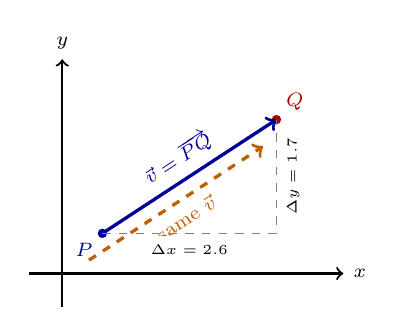
\begin{tikzpicture}[scale=0.85,every node/.style={font=\scriptsize}]
  \draw[->,thick] (-0.5,0)--(4.2,0) node[right] {$x$};
  \draw[->,thick] (0,-0.5)--(0,3.2) node[above] {$y$};
  \fill[blue!60!black] (0.6,0.6) circle (2pt) node[below left] {$P$};
  \fill[red!70!black] (3.2,2.3) circle (2pt) node[above right] {$Q$};
  \draw[->,very thick,blue!60!black] (0.6,0.6)--(3.2,2.3) node[midway,above,sloped] {$\vec{v}=\overrightarrow{PQ}$};
  \draw[->,very thick,orange!75!black,dashed] (0.4,0.2)--(3.0,1.9) node[midway,below,sloped] {same $\vec{v}$};
  \draw[dashed,gray] (0.6,0.6)--(3.2,0.6)--(3.2,2.3);
  \node[font=\tiny,fill=white] at (1.9,0.35) {$\Delta x=2.6$};
  \node[font=\tiny,fill=white,rotate=90] at (3.45,1.45) {$\Delta y=1.7$};
\end{tikzpicture}
\caption{A vector as a free arrow. $\overrightarrow{PQ}$ and its translate have the same components $(\Delta x,\Delta y)$.}
\label{fig:free-vector}
\end{figure}

\begin{definition}[Vector in $\mathbb{R}^n$]
A \emph{vector} $\mathbf{v}\in\mathbb{R}^n$ is an ordered $n$-tuple
\[
  \mathbf{v}=\begin{bmatrix}v_1\\v_2\\\vdots\\v_n\end{bmatrix},\quad v_i\in\mathbb{R}.
\]
We write $\mathbf{0}$ for the zero vector and $-\mathbf{v}$ for the opposite arrow. Two arrows represent the same vector iff their component differences agree.
\end{definition}

Addition is tip-to-tail; scalar multiplication stretches.

\begin{figure}[h]
\centering
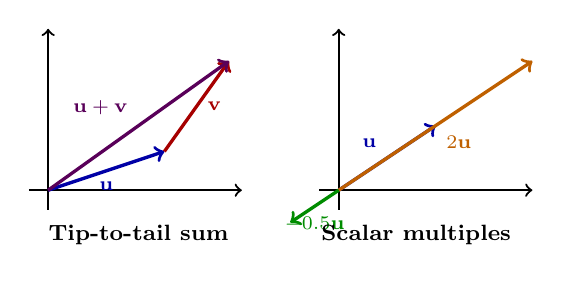
\begin{tikzpicture}[scale=0.82,every node/.style={font=\scriptsize}]
  \begin{scope}
    \draw[->,thick] (-0.3,0)--(3.0,0); \draw[->,thick] (0,-0.3)--(0,2.5);
    \draw[->,very thick,blue!65!black] (0,0)--(1.8,0.6) node[midway,below] {$\mathbf{u}$};
    \draw[->,very thick,red!65!black] (1.8,0.6)--(2.8,2.0) node[midway,right] {$\mathbf{v}$};
    \draw[->,very thick,violet!70!black] (0,0)--(2.8,2.0) node[midway,above left] {$\mathbf{u}+\mathbf{v}$};
    \node[font=\footnotesize\bfseries] at (1.4,-0.7) {Tip-to-tail sum};
  \end{scope}
  \begin{scope}[xshift=4.5cm]
    \draw[->,thick] (-0.3,0)--(3.0,0); \draw[->,thick] (0,-0.3)--(0,2.5);
    \draw[->,very thick,blue!65!black] (0,0)--(1.5,1.0) node[midway,above left] {$\mathbf{u}$};
    \draw[->,very thick,orange!75!black] (0,0)--(3.0,2.0) node[midway,below right] {$2\mathbf{u}$};
    \draw[->,very thick,green!55!black] (0,0)--(-0.75,-0.5) node[midway,below] {$-0.5\mathbf{u}$};
    \node[font=\footnotesize\bfseries] at (1.2,-0.7) {Scalar multiples};
  \end{scope}
\end{tikzpicture}
\caption{Left: $\mathbf{u}+\mathbf{v}$ (parallelogram rule). Right: $c\mathbf{u}$ scales length by $|c|$, flips if $c<0$.}
\label{fig:add-scale}
\end{figure}

Algebraically,
\[
  \mathbf{u}+\mathbf{v}=\begin{bmatrix}u_1+v_1\\\vdots\\u_n+v_n\end{bmatrix},\quad
  c\mathbf{u}=\begin{bmatrix}cu_1\\\vdots\\cu_n\end{bmatrix}.
\]
Properties: commutativity, associativity, distributivity --- all inherited from $\mathbb{R}$.

\section{Length, Dot Product, and Angle}
\label{sec:dot}
How long is an arrow? Pythagoras in $n$ dimensions.

\begin{definition}[Norm and dot product]
For $\mathbf{u},\mathbf{v}\in\mathbb{R}^n$,
\[
  \mathbf{u}\cdot\mathbf{v}=u_1v_1+\cdots+u_nv_n,\qquad
  \|\mathbf{u}\|=\sqrt{\mathbf{u}\cdot\mathbf{u}}=\sqrt{u_1^2+\cdots+u_n^2}.
\]
Distance between tips: $\|\mathbf{u}-\mathbf{v}\|$.
\end{definition}

\begin{theorem}[Cauchy--Schwarz and angle]
For any $\mathbf{u},\mathbf{v}$,
\[
  |\mathbf{u}\cdot\mathbf{v}|\le\|\mathbf{u}\|\,\|\mathbf{v}\|,
\]
with equality iff one is a scalar multiple of the other. If both nonzero, there is a unique $\theta\in[0,\pi]$ with
\[
  \mathbf{u}\cdot\mathbf{v}=\|\mathbf{u}\|\,\|\mathbf{v}\|\cos\theta,
\]
and $\theta$ is the geometric angle between them.
\end{theorem}
\begin{proof}[Sketch]
Consider $\|\mathbf{u}-t\mathbf{v}\|^2\ge0$ for all $t\in\mathbb{R}$; its discriminant must be $\le0$, giving Cauchy--Schwarz. Define $\theta$ via $\cos\theta=(\mathbf{u}\cdot\mathbf{v})/(\|\mathbf{u}\|\|\mathbf{v}\|)$.
\end{proof}

Corollary: $\mathbf{u}\perp\mathbf{v}$ (orthogonal) iff $\mathbf{u}\cdot\mathbf{v}=0$.

\begin{figure}[h]
\centering
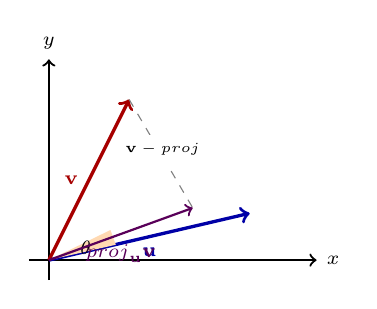
\begin{tikzpicture}[scale=0.85,every node/.style={font=\scriptsize}]
  \draw[->,thick] (-0.3,0)--(4.0,0) node[right] {$x$};
  \draw[->,thick] (0,-0.3)--(0,3.0) node[above] {$y$};
  \draw[->,very thick,blue!65!black] (0,0)--(3.0,0.7) node[midway,below] {$\mathbf{u}$};
  \draw[->,very thick,red!65!black] (0,0)--(1.2,2.4) node[midway,left] {$\mathbf{v}$};
  \draw[dashed,gray] (1.2,2.4)--(2.15,0.78);
  \fill[orange!30] (0,0)--(1.0,0.23)--(0.92,0.45)--cycle;
  \node at (0.55,0.18) {$\theta$};
  \draw[->,thick,violet!70!black] (0,0)--(2.15,0.78) node[midway,below] {$\operatorname{proj}_{\mathbf{u}}\mathbf{v}$};
  \node[font=\tiny,fill=white] at (1.7,1.65) {$\mathbf{v}-\operatorname{proj}$};
\end{tikzpicture}
\caption{Angle $\theta$ via the dot product; projection of $\mathbf{v}$ onto $\mathbf{u}$ is the shadow along $\mathbf{u}$.}
\label{fig:angle-proj}
\end{figure}

\emph{Projection:} the shadow of $\mathbf{v}$ on $\mathbf{u}\neq\mathbf{0}$ is
\[
  \operatorname{proj}_{\mathbf{u}}\mathbf{v}=\frac{\mathbf{v}\cdot\mathbf{u}}{\mathbf{u}\cdot\mathbf{u}}\,\mathbf{u},\qquad
  \|\operatorname{proj}_{\mathbf{u}}\mathbf{v}\|= \|\mathbf{v}\|\,|\cos\theta|.
\]
Useful everywhere from graphics (shadows) to ML (closest point).

\begin{example}[Cosine similarity]
In text retrieval, documents are vectors of word counts. $\cos\theta=(\mathbf{a}\cdot\mathbf{b})/(\|\mathbf{a}\|\|\mathbf{b}\|)$ near $1$ means similar topics --- the same formula as geometry.
\end{example}

\section{Lines and Planes}
\label{sec:lines-planes}
A line is a point plus a direction. A plane is a point plus two independent directions.

\begin{align}
  \text{Line: } &\mathbf{x}=\mathbf{p}+t\mathbf{d},\quad t\in\mathbb{R},\\
  \text{Plane in $\mathbb{R}^3$: } &\mathbf{x}=\mathbf{p}+s\mathbf{d}_1+t\mathbf{d}_2,\quad s,t\in\mathbb{R},\\
  \text{Plane (normal form): } &\mathbf{n}\cdot(\mathbf{x}-\mathbf{p})=0\iff \mathbf{n}\cdot\mathbf{x}=d.
\end{align}
Here $\mathbf{d}$ is a direction vector and $\mathbf{n}$ is a \emph{normal} (perpendicular) vector. In $\mathbb{R}^3$, if $\mathbf{d}_1,\mathbf{d}_2$ span the plane then $\mathbf{n}=\mathbf{d}_1\times\mathbf{d}_2$ (cross product).

\begin{example}[Distance from point to line]
Let $L:\mathbf{p}+t\mathbf{d}$. For $\mathbf{q}$, let $\mathbf{w}=\mathbf{q}-\mathbf{p}$. Then
\[
  \text{dist}(\mathbf{q},L)=\left\|\mathbf{w}-\operatorname{proj}_{\mathbf{d}}\mathbf{w}\right\|
  =\frac{\|\mathbf{w}\times\mathbf{d}\|}{\|\mathbf{d}\|}\quad(\text{in }\mathbb{R}^3).
\]
Subtract the along-line shadow; what remains is the perpendicular distance.
\end{example}

\begin{example}[Python --- vectors as arrays]
\begin{lstlisting}[language=Python]
import numpy as np
u = np.array([3.0, 1.0])
v = np.array([1.0, 2.0])
dot = u @ v                      # 5.0
norm_u = np.linalg.norm(u)       # sqrt(10)
cos_theta = dot/(norm_u*np.linalg.norm(v))
proj = (dot/(u@u))*u             # projection of v onto u? careful: swap
proj_v_on_u = (v@u)/(u@u) * u
print(cos_theta, proj_v_on_u)
\end{lstlisting}
\end{example}

% ============================================================

% --- Additional depth: Cross product and applications ---
\section{Cross Product and Volume}
\label{sec:cross}
In $\mathbb{R}^3$, the \emph{cross product} $\mathbf{u}\times\mathbf{v}$ is the vector orthogonal to both $\mathbf{u},\mathbf{v}$ with magnitude $\|\mathbf{u}\|\|\mathbf{v}\|\sin\theta$ (area of the parallelogram) and direction by the right-hand rule.
\[
  \mathbf{u}\times\mathbf{v}=\begin{bmatrix}u_2v_3-u_3v_2\\u_3v_1-u_1v_3\\u_1v_2-u_2v_1\end{bmatrix},\quad
  \|\mathbf{u}\times\mathbf{v}\|=\|\mathbf{u}\|\|\mathbf{v}\|\sin\theta.
\]
Properties: $\mathbf{u}\times\mathbf{v}=-(\mathbf{v}\times\mathbf{u})$, $\mathbf{u}\times\mathbf{u}=\mathbf{0}$, bilinear. The scalar triple product $\mathbf{u}\cdot(\mathbf{v}\times\mathbf{w})=\det[\mathbf{u}\ \mathbf{v}\ \mathbf{w}]$ is the signed volume.

\begin{example}[Normal to a plane]
Points $P(1,0,0),Q(0,1,0),R(0,0,1)$: $\overrightarrow{PQ}=[-1,1,0]^T$, $\overrightarrow{PR}=[-1,0,1]^T$, so $\mathbf{n}=\overrightarrow{PQ}\times\overrightarrow{PR}=[1,1,1]^T$. Plane: $x+y+z=1$, matching $\mathbf{n}\cdot(\mathbf{x}-P)=0$.
\end{example}

\section{Inequalities and Geometry}
\label{sec:inequalities}
Two inequalities govern all distance arguments:
\begin{theorem}[Triangle and Cauchy--Schwarz]
For $\mathbf{u},\mathbf{v}\in\mathbb{R}^n$: (i) $\|\mathbf{u}+\mathbf{v}\|\le\|\mathbf{u}\|+\|\mathbf{v}\|$ (triangle), equality when $\mathbf{u},\mathbf{v}$ same direction; (ii) $|\mathbf{u}\cdot\mathbf{v}|\le\|\mathbf{u}\|\|\mathbf{v}\|$ with equality iff dependent.
\end{theorem}
Triangle follows from $\|\mathbf{u}+\mathbf{v}\|^2=\|\mathbf{u}\|^2+2\mathbf{u}\cdot\mathbf{v}+\|\mathbf{v}\|^2\le(\|\mathbf{u}\|+\|\mathbf{v}\|)^2$ via Cauchy--Schwarz. These justify calling $\|\cdot\|$ a norm and $d(\mathbf{u},\mathbf{v})=\|\mathbf{u}-\mathbf{v}\|$ a metric.


\section{Chapter Notes}
Vectors go back to Grassmann and Gibbs; modern computing treats them as arrays. The dot product as $\|\mathbf{u}\|\|\mathbf{v}\|\cos\theta$ unifies algebra and geometry --- the bridge used in graphics, robotics, and embeddings.

% ============================================================
\section{Exercises}
\label{sec:ch01-exercises}
\begin{enumerate}[label=E1.\arabic*, leftmargin=*, itemsep=0.8em]
\item \textbf{Arithmetic.} Let $\mathbf{u}=[2,-1,3]^T$, $\mathbf{v}=[0,2,-1]^T$. Compute $\mathbf{u}+\mathbf{v}$, $3\mathbf{u}-2\mathbf{v}$, $\mathbf{u}\cdot\mathbf{v}$, $\|\mathbf{u}\|$, and the angle $\theta$ between $\mathbf{u}$ and $\mathbf{v}$ (to $1^\circ$).
\item \textbf{Orthogonality.} Find all $c$ such that $[c,2,1]^T$ is orthogonal to $[1,c,-2]^T$. Give a geometric interpretation of your answer.
\item \textbf{Line and distance.} Let $L:\mathbf{p}=[1,0,2]^T$, $\mathbf{d}=[1,1,1]^T$. Write the parametric equation, find the point on $L$ closest to $\mathbf{q}=[2,3,0]^T$, and compute $\text{dist}(\mathbf{q},L)$.
\item \textbf{Projection proof.} Prove $\mathbf{v}-\operatorname{proj}_{\mathbf{u}}\mathbf{v}$ is orthogonal to $\mathbf{u}$. Use this to derive the formula for distance from a point to a plane $\mathbf{n}\cdot\mathbf{x}=d$ in $\mathbb{R}^3$.
\item \textbf{Coding.} Write a Python function \texttt{gram\_schmidt\_2(u,v)} returning an orthonormal pair spanning the same plane as $\mathbf{u},\mathbf{v}$ (assume independent). Test on $\mathbf{u}=[1,1,0]^T$, $\mathbf{v}=[1,0,1]^T$ and verify orthonormality numerically.
\end{enumerate}
% End of Chapter 1
